% \begin{subappendices}

%     \section{Supplementary Information}

\begin{ThreePartTable}
     \begin{TableNotes}
         \item[a] Taken from Gaussian fit of relative depletion spectrum (not power normalized).\\
         \item[b] Taken from Gaussian fit of power normalized spectrum.\\
         \item[c] Estimated from power normalized spectrum: fitting was problematic in the power normalized spectrum in this region due to the high noise level as a result of the relatively low power.  
     \end{TableNotes}
    \begin{longtable}{*{16}{c}}
        \caption{Observed band centers and intensities in the IRPD spectrum of \ion tagged with Ne obtained from fitting Gaussian functions to the experimental data in both  relative depletion and power normalized intensity units (see main text). The frequency error is dominated by the calibration method using either a grating spectrometer (FEL) or a wavemeter (OPO). }\label{tab:obs_lines}\\
        
        \toprule
       \textbf{Freq. (\wn)} \tnote{a} & \textbf{Freq. err. (\wn)} & \textbf{Norm. Int. (rel.u)}\tnote{b} &  \textbf{Norm. Int. err. (rel.u)}\tnote{b}\\
        
        \midrule
        \endfirsthead
        \\\\\hline \multicolumn{8}{c}{{\bfseries \tablename\ \thetable{} -- continued from previous page}} \\
        \toprule
        \textbf{Freq. (\wn)} \tnote{a} & \textbf{Freq. err. (\wn)} & \textbf{Norm. Int. (rel.u)}\tnote{b} &  \textbf{Norm. Int. err. (rel.u)}\tnote{b}\\
    
        \toprule
        \endhead
    
        \midrule
        \insertTableNotes
        \\\\\hline \multicolumn{8}{c}{{\bfseries \tablename\ \thetable{} -- continued on next page}} \\ \hline
        \endfoot
        \bottomrule
        \insertTableNotes
        \endlastfoot

    189     &	2    &		1.6 \tnote{c}  &	-\\
    200     &	3    &		1.6 \tnote{c}  &	-\\
    208     &	3    &		1.6 \tnote{c}  &	-\\
    231     &	2    &		1.4 \tnote{c}  &	-\\
    238     &	1    &		3.4        &	0.5\\
    384     &	1    &		0.9        &	0.3\\
    439     &	1    &	    12.1       &	0.3\\
    454     &	1    &	    9.9        &	0.3\\
    489     &	1    &	    2.5        &	0.3\\
    552     &	2    &	    0.6        &	0.2\\
    572     &	2    &	    0.7        &	0.2\\
    626     &	1    &	    13.2       &	0.5\\
    631     &	1    &		5.7        &	0.4\\
    688     &	1    &		15.4       &	0.2\\
    704     &	1    &		5.0        &	0.2\\
    846     &	1    &	    4.9        &	0.2\\
    926     &	1    &	    0.6        &	0.2\\
    957     &	1    &	    2.2        &	0.2\\
    981     &	2    &	    0.5        &	0.2\\
    1097    &	1    &	    0.2        &	0.2\\
    1243    &	1    &	    1.1        &	0.3\\
    1253    &	1    &	    1.0        &	0.5\\
    1331    &	1    &	    0.6        &	0.3\\
    1595    &	1    &		1.1        &	0.2\\
    1845    &	1    &	    35.9       &	0.2\\
    2171    &	1    &	    8.8        &	0.2\\
    3174.0  &   1    &      5.4        &    0.4\\
    3182.9	&   0.5	 &      16	       &    2\\
    3184.7	&   0.5  &      19         &	2\\
    3185.7  &   0.5	 &      22         &	1\\
    3191.9	&   0.5	 &      20         &	4\\
    3195.2	&   0.5	 &      28	       &    3\\	

\end{longtable}
\end{ThreePartTable}
\clearpage

\begin{figure}
    \centering
    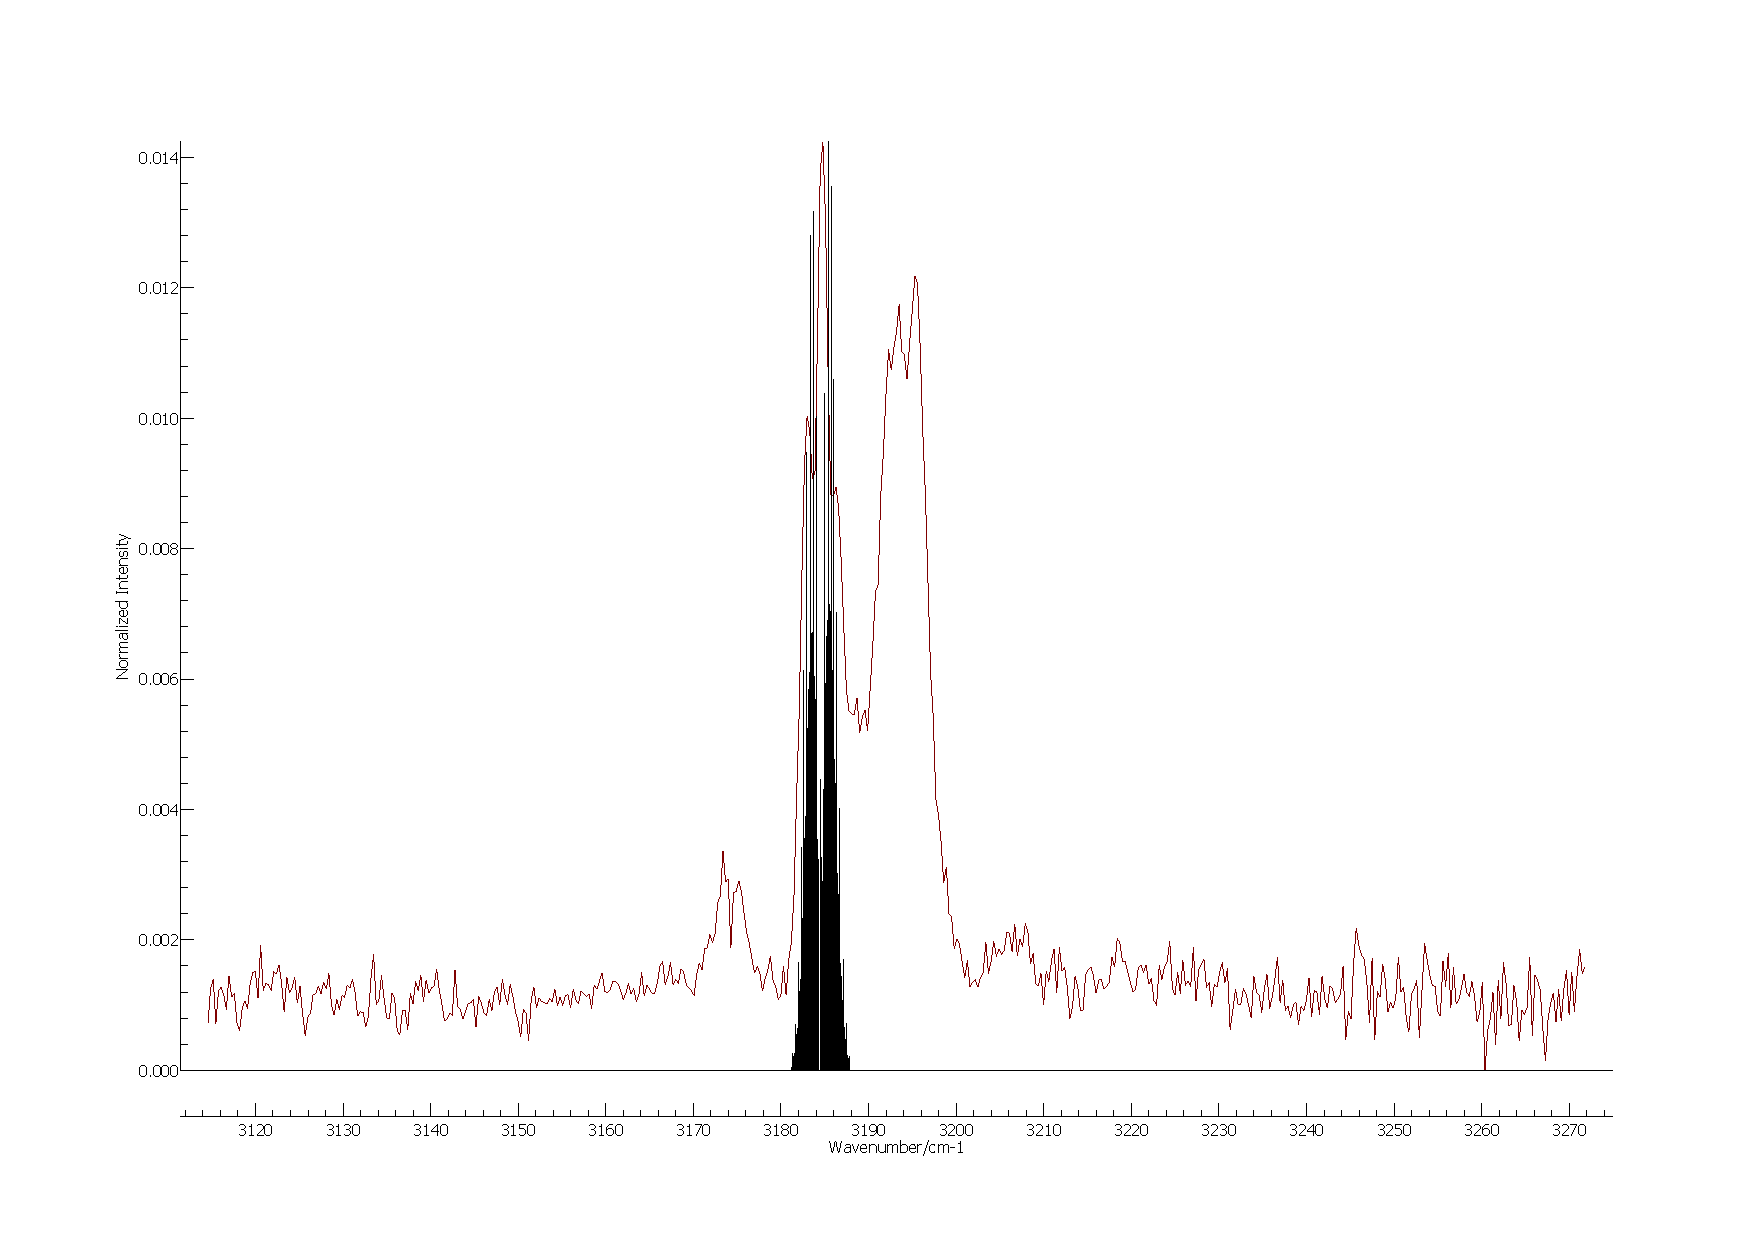
\includegraphics[width=\textwidth,height=\textheight,keepaspectratio]{chapters/HC3N+/figures/spectrum/PGOPHER_HC3N+.pdf}
    \caption{IRPD spectrum of the HC$_3$N$^+$ ion tagged with Ne in the range 3120-3260 cm$^{-1}$ recorded with an OPO (red) overlayed with a prediction of the $\nu_1$ ro-vibrational structure using the PGOPHER program package \cite{western_pgopher_2017} (black, $T$=20 K and $B$ = 0.033 cm$^{-1}$, calculated at RCCSD(T)/cc-pVTZ level of theory).}
    \label{fig:PGopher}
\end{figure}


\begin{longtable}[!h] {p{.15\textwidth} p{.15\textwidth} p{.08\textwidth} p{.08\textwidth} p{.08\textwidth} p{.08\textwidth} p{.08\textwidth} p{.08\textwidth}}
    
    \caption{Calculated frequencies and intensities based on \emph{ab initio} parameters of \citet{Dai2015TheCalculations} together with the assigned $P$ and $K$ quantum numbers and the population in the $\nu_5$, $\nu_6$ and $\nu_7$ bending modes}
    \label{tab:ab_initio_freq}\\

    \hline\hline \multicolumn{1}{p{.15\textwidth}}{\textbf{Freq (\wn)}}   &	\multicolumn{1}{p{.15\textwidth}}{\textbf{Rel. Int (a.u.)}}	&   \multicolumn{1}{p{.08\textwidth}}{${\bm K}$}	&   \multicolumn{1}{p{.08\textwidth}}{$\bm{P}$}    & 	\multicolumn{1}{p{.08\textwidth}}{\textbf{pop $\nu_5$}}  & 	\multicolumn{1}{p{.08\textwidth}}{\textbf{pop $\nu_6$}}   & 	\multicolumn{1}{p{.08\textwidth}}{\textbf{pop $\nu_7$}}   & 	\multicolumn{1}{p{.08\textwidth}}{\textbf{pop tot}}\\
    \hline
    \endfirsthead
    
    \multicolumn{8}{c}%
    {{\bfseries \tablename\ \thetable{} -- continued from previous page}} \\
    \hline\hline \multicolumn{1}{p{.15\textwidth}}{\textbf{Freq (\wn)}}   &	\multicolumn{1}{p{.15\textwidth}}{\textbf{Rel. Int (a.u.)}}	&   \multicolumn{1}{p{.08\textwidth}}{\textbf{K}}	&   \multicolumn{1}{p{.08\textwidth}}{\textbf{P}}    & 	\multicolumn{1}{p{.08\textwidth}}{\textbf{pop $\nu_5$}}  & 	\multicolumn{1}{p{.08\textwidth}}{\textbf{pop $\nu_6$}}   & 	\multicolumn{1}{p{.08\textwidth}}{\textbf{pop $\nu_7$}}   & 	\multicolumn{1}{p{.08\textwidth}}{\textbf{pop tot}}\\
    \hline
    \endhead
    
    \hline \multicolumn{8}{c}{{continued on next page}} \\ \hline
    \endfoot
    
    \hline \hline 
    \endlastfoot
    
    190.77  &   0.0423  & 	0   & 	0.5  &	0.02 &	0.01 &	0.99 &	1.02\\
    195.46  &	0.0443  &	2   &	2.5  &	0.01 &	0.01 &	1.01 &	1.03\\
    237.33  &	0.132   &	0   &	0.5  &	0.02 &	0.02 &  0.98 &	1.02\\
    238.17  &	0       &	2   &	1.5	 &  0.02 &	0.01 &	1.01 &	1.04\\
    382.26  & 	0       &	1   &	0.5	 &  0.02 &	0.02 &	1.98 &	2.02\\
    383.77  &	0       &	1   &	1.5  &	0.02 &	0.01 &	2    &	2.03\\
    431.86  &	0       &	1   &	1.5  &	0.03 &	0.04 &	1.96 &	2.03\\
    434.43  &	0       &	1   &	0.5  &	0.03 &	0.02 &	1.98 &	2.03\\
    446.02  &	0.0727  &	0   &	0.5	 &  0.04 &	0.97 &	0.02 &	1.03\\
    457.8   &	0.081   &	2   &	2.5	 &  0.01 &	1.01 &	0.01 &	1.03\\
    496.53  &	0.3849  &	0   &	0.5  &	0.17 &	0.83 &	0.02 &	1.02\\
    500.45  &	0.0084  &	2   &	1.5  &	0.02 &	1.01 &	0.01 &	1.04\\
    573.56  &   0.0051  &	0   &	0.5  &	0.02 &	0.02 &	2.99 &	3.03\\
    574.26  &   0.0004  &	2   &	1.5	 &  0.02 &  0.02 &	2.97 &	3.01\\
    576.7   &	0.0046  &	2   &	2.5  &	0.02 &	0.02 &	3    &	3.04\\
    626.58  &	0.0088  &	2   &	2.5  &	0.04 &	0.05 &	2.94 &	3.03\\
    629.6   &	0.7167  &	0	&   0.5  &	0.84 &	0.17 &	0.02 &	1.03\\
    630.58  &	0.0514  &	0   &	0.5	 &  0.04 &  0.04 &  2.94 &	3.02\\
    631.05  &	0       &	2   &	1.5  &	0.03 &	0.03 &	2.98 &	3.04\\
    639.03  &   0       &	1   &	0.5	 &  0.04 &	0.97 &	1.01 &	2.02\\
    640.54  &   0       &	1   &	1.5	 &  0.03 &	0.99 &	1.01 &	2.03\\
    649.84  &	0       &	1   &	1.5	 & 	0.03 &	0.99 &	1    &	2.02\\
    688.74  &	0       &	1   &	0.5	 & 	0.05 &	1    &	0.98 &	2.03\\
    694.18  &	0       &	1   &	1.5	 & 	0.16 &	0.85 &	1.01 &	2.02\\
    696.79  &	0       &	1   &	0.5	 & 	0.14 &	0.87 &	1.02 &	2.03\\
    697.87  &	1       &	2   &	2.5	 & 	1.03 &	0.01 &	0.01 &	1.05\\
    739.89  &	0       &	2   &	1.5	 & 	1.04 &	0.01 &	0.01 &	1.06\\
    823.55  &	0       &	1   &	1.5	 & 	0.85 &	0.18 &	0.99 &	2.02\\
    824.04  &	0       &	1   &	0.5	 & 	0.85 &	0.17 &	1    &	2.02\\
    830.01  &	0.0027  &	0   &	0.5	 & 	0.03 &	1    &	2    &	3.03\\
    832.29  &	0.0006  &	2   &	1.5	 & 	0.04 &	0.98 &	2    &	3.02\\
    833.64  &	0.003   &	2   &	2.5	 & 	0.03 &	1    &	2.01 &	3.04\\
    840.86  &	0.0132  &	0   &	0.5	 & 	0.04 &	1    &	1.99 &	3.03\\
    847.01  &	0.0105  &	2   &	2.5	 & 	0.04 &	0.98 &	2.02 &	3.04\\
    875.36  &	0.5467  &	0   &	0.5	 & 	0.93 &	0.09 &	0.14 &	1.16\\
    880.22  &	0.1438  &	0   &	0.5	 & 	0.11 &	0.98 &	1.81 &	2.9\\
    883.97  &	0       &	2   &	1.5	 & 	0.05 &	1.01 &	1.99 &	3.05\\
    887.72  &	0       &	1   &	1.5	 & 	0.94 &	0.22 &	0.89 &	2.05\\
    891.73  &	0       &	2   &	2.5	 & 	0.15 &	0.87 &	2    &	3.02\\
    895.48  &	0.0012  &	0   &	0.5	 & 	0.15 &	0.87 &	2.01 &	3.03\\
    895.59  &	0       &	1   &	0.5	 & 	0.06 &	1.93 &	0.03 &	2.02\\
    895.62  &	0       &	2   &	1.5	 & 	0.14 &	0.86 &	2.03 &	3.03\\
    897.55  &	0       &	1   &	1.5	 & 	0.13 &	1.78 &	0.12 &	2.03\\
    927.01  &	0       &	1   &	0.5	 & 	1    &	0.14 &	0.9  &	2.04\\
    952.36  &	0       &	1   &	1.5	 &	0.26 &	1.72 &	0.05 & 	2.03\\
    959.59  &	0       &	1   &	0.5	 &	0.26 &	1.67 &	0.11 &	2.04\\
    1016.86 &	0.0031  &	0   &	0.5	 &	0.86 &	0.17 &	1.99 &	3.02\\
    1017.8  &	0.0044  &	2   &	2.5	 &	0.87 &	0.18 &	1.99 &	3.04\\
    1018.63 &	0       &	2   &	1.5	 &	0.86 &	0.17 &	2    &	3.03\\
    1065.54 &	0       &	1   &	1.5	 &	0.94 &	0.17 &	1.06 &	2.17\\
    1069.42 &	0       &	1   &	0.5	 &	0.96 &	0.09 &	1.05 &	2.1\\
    1077.95 &	0.003   &	0   &	0.5	 &	0.85 & 	0.43 &	1.76 &	3.04\\
    1083.01 &	0.0032  &	2	&   2.5	 &	0.98 &	0.14 &	1.94 &	3.06\\
    1088.09 &	0.0052	&   0	&   0.5	 &	0.23 &	1.6  &	1.2  &	3.03\\
    1089.7  &	0       &	2	&	1.5	 &	0.06 &	1.94 &	1.02 &	3.02\\
    1090.94 &	0.0013	&	2	&   2.5  &	0.09 &	1.87 &	1.07 &	3.03\\
    1094.39 &	0       &	1	&	0.5	 &	0.77 &	1.17 &	0.23 &	2.17\\
    1097.24 &	0       &	1	&	1.5	 &	0.79 &	1.22 & 	0.02 &	2.03\\
    1097.4  &	0.0045  &	0	&	0.5	 &	0.08 &	1.89 &	1.06 &	3.03\\
    1104.7  &	0.0025  &	2	&	2.5	 &	0.04 &	2    &	1    &	3.04\\
    1116.79 &	0.0025  &	0	&	0.5	 &	1    &	0.18 &	1.86 &	3.04\\
    1121.83 &	0       &	2	&	1.5	 &	1.02 & 	0.12 &	1.93 &	3.07\\
    1142.98 &	0       &	2	&	1.5	 &	0.05 &	2.03 &	0.97 &	3.05\\
    1144.64 &	0       &	1	&	1.5	 &	1.14 &	0.79 &	0.11 &	2.04\\
    1150.29 &	0.0057  &	0	&	0.5	 &	0.25 & 	1.7  &	1.08 &	3.03\\
    1151.33 &	0.0037  &	2	&	2.5	 &	0.25 & 	1.74 &	1.04 &	3.03\\
    1157.74 &	0       &	2	&	1.5	 &	0.23 &	1.73 &	1.09 &	3.05\\
    1158.66 &	0.0013  &	0	&	0.5	 &	0.25 &	1.71 &	1.08 &	3.04\\
    1171.57 &	0       &	1	&	0.5	 &	1.26 & 	0.73 &	0.06 &	2.05\\
    1256.75 &	0.0037  &	2	&	2.5	 &	0.96 &	0.21 &	1.99 &	3.16\\
    1259.34 &	0.0012  &	0	&	0.5	 &	0.98 &	0.18 &	1.93 &	3.09\\
    1263.41 &	0       &	2	&	1.5	 &	0.98 &	0.11 &	2    &	3.09\\
    1270.56 &	0       &	1	&	1.5	 &	1.72 &	0.29 &	0.05 &	2.06\\
    1285.89 &	0.0004  &	0	&	0.5	 &	0.83 &	1.2  &	1    &	3.03\\
    1287.75 &	0       &	1	&	0.5	 &	1.62 &	0.39 &	0.04 &	2.05\\
    1287.92 &	0       &	2	&	1.5	 &	0.82 &	1.19 &	1.05 &	3.06\\
    1289.36 &	0.0027  &	2	&	2.5	 &	0.81 &	1.23 &	0.99 &	3.03\\
    1291.39 &	0.0008  &	0	&	0.5	 &	0.82 &	1.21 &	1.02 &	3.05\\
    1337.46 &	0.0064  &	0	&	0.5	 &	0.83 &	1.39 &	0.81 &	3.03\\
    1339.32 &	0.0013  &	2	&	2.5	 &	0.9  &	1.3  &	0.85 &	3.05\\
    1344.8  &	0.005   &	0	&	0.5	 &	0.38 &	2.31 &	0.34 &	3.03\\
    1346.92 &	0       &	2	&	1.5	 &	0.07 &	2.91 &	0.05 &	3.03\\
    1346.99 &	0.0033  &	2	&	2.5	 &	1.02 &	0.97 &	1.06 &	3.05\\
    1349.2  &	0.0001  &	2	&	2.5	 &	0.28 &	2.48 &	0.27 &	3.03\\
    1350.4  &	0       &	1	&	0.5	 &	1.11 &	0.91 &	0.03 &	2.05\\
    1353.66 &	0       &	1	&	1.5	 &	1.09 &	0.93 &	0.09 &	2.11\\
    1366.31 &	0.0014  &	0	&	0.5	 &	1.18 &	0.84 &	1.02 &	3.04\\
    1370.89 &	0       &	2	&	1.5	 &	1.23 & 	0.74 &	1.09 &	3.06\\
    1377.57 &	0       &	2	&	1.5	 &	1.02 &	1.15 &	0.89 &	3.06\\
    1409.08 &	0.0012  &	2	&	2.5	 &	0.32 &	2.64 &	0.07 &	3.03\\
    1415.93 &	0.0003  &	0	&	0.5	 &	0.36 &	2.59 &	0.09 &	3.04\\
    1420.3  &	0       &	2	&	1.5	 &	0.3  &	2.61 &	0.14 &	3.05\\
    1464.62 &	0.001   &	0	&	0.5	 &	1.58 &	0.38 &	1.35 &	3.31\\
    1467.83 &	0.0003  &	2	&	2.5	 &	1.41 &	0.53 &	1.56 &	3.5\\
    1483.97 &	0       &	2	&	1.5	 &	1.42 &	0.6  &	1.34 &	3.36\\
    1485.88 &	0.0017  &	0	&	0.5	 &	1.61 &	0.44 & 	1.03 &	3.08\\
    1529.41 &	0.0009  &	0	&	0.5	 &	1.13 &	1.2  &	0.76 &	3.09\\
    1539.79 &	0.0013  &	0	&	0.5	 &	1.11 &	1.1  &	0.89 &	3.1\\
    1539.97 &	0.0015  &	2	&	2.5	 &	1.1  &	1.09 &	0.97 &	3.16\\
    1542.3  &	0       &	2	&	1.5	 &	1.11 &	0.98 &	0.99 &	3.08\\
    1558.24 &	0       &	2	&	1.5	 &	0.76 &	2.16 &	0.24 &	3.16\\
    1562.27 &	0.0015  &	2	&	2.5	 &	0.8  &	2.16 &	0.07 &	3.03\\
    1562.55 &	0.0019  &	0	&	0.5	 &	0.8  &	2.01 &	0.26 &	3.07\\
    1578.58 &	0.0026  &	2	&	2.5	 &	2    &	0.13 &	0.94 &	3.07\\
    1596.91 &	0       &	0	&	0.5	 &	1.17 &	1.62 &	0.26 &	3.05\\
    1606.17 &	0.0019  &	2	&	2.5	 &	1.18 &	1.69 &	0.19 &	3.06\\
    1612.81 &	0       &	2	&	1.5	 &	1.89 &	0.45 &	0.74 &	3.08\\
    1615.51 &	0.0014  &	0	&	0.5	 &	1.33 &	1.59 &	0.13 &	3.05\\
  
    \end{longtable}


\begin{longtable}[!h] {p{.15\textwidth} p{.15\textwidth} p{.08\textwidth} p{.08\textwidth} p{.08\textwidth} p{.08\textwidth} p{.08\textwidth} p{.08\textwidth}}
    
    \caption{Same as Table \ref{tab:ab_initio_freq}, but calculated based on fitted spectroscopic parameters of the IRPD spectrum, all given in \wn: $\omega_5$ = 699, $g_{55}$ = 115, $g_{56} = -50$, $\omega_6 $ = 455, $g_{66} = -23$, $g_{57} = -34.72$, $\omega_7$ = 198, $g_{77} = -14$, $g_{67}$ = 15, $A_{SO} = -44.$}
    \label{tab:fit_freq}\\

    \hline\hline \multicolumn{1}{p{.15\textwidth}}{\textbf{Freq (\wn)}}   &	\multicolumn{1}{p{.15\textwidth}}{\textbf{Rel. Int (a.u.)}}	&   \multicolumn{1}{p{.08\textwidth}}{$\bm K$}	&   \multicolumn{1}{p{.08\textwidth}}{$\bm{P}$}    & 	\multicolumn{1}{p{.08\textwidth}}{\textbf{pop $\nu_5$}}  & 	\multicolumn{1}{p{.08\textwidth}}{\textbf{pop $\nu_6$}}   & 	\multicolumn{1}{p{.08\textwidth}}{\textbf{pop $\nu_7$}}   & 	\multicolumn{1}{p{.08\textwidth}}{\textbf{pop tot}}\\
    \hline
    \endfirsthead
    
    \multicolumn{8}{c}%
    {{\bfseries \tablename\ \thetable{} -- continued from previous page}} \\
    \hline\hline \multicolumn{1}{p{.15\textwidth}}{\textbf{Freq (\wn)}}   &	\multicolumn{1}{p{.15\textwidth}}{\textbf{Rel. Int (a.u.)}}	&   \multicolumn{1}{p{.08\textwidth}}{$\bm{K}$}	&   \multicolumn{1}{p{.08\textwidth}}{$\bm{P}$}    & 	\multicolumn{1}{p{.08\textwidth}}{\textbf{pop $\nu_5$}}  & 	\multicolumn{1}{p{.08\textwidth}}{\textbf{pop $\nu_6$}}   & 	\multicolumn{1}{p{.08\textwidth}}{\textbf{pop $\nu_7$}}   & 	\multicolumn{1}{p{.08\textwidth}}{\textbf{pop tot}}\\
    \hline
    \endhead
    
    \hline \multicolumn{8}{c}{{continued on next page}} \\ \hline
    \endfoot
    
    \hline \hline 
    \endlastfoot
    
	190.26	&	0.0399	&	0	&	0.5	&	0.01	&	0.01	&	1		&	1.02	\\
	195.14	&	0.0138	&	2	&	2.5	&	0.01	&	0		&	1.01	&	1.02    \\
	238.09	&	0.0399	&	2	&	1.5	&	0.01	&	0		&	1.01	&	1.02    \\
	240.07	&	0.1296	&	0	&	0.5	&	0.02	&	0.01	&	0.99	&	1.02    \\
	381.43	&	0		&	1	&	0.5	&	0.02	&	0.01	&	1.99	&	2.02    \\
	382.02	&	0		&	1	&	1.5	&	0.01	&	0.01	&	2		&	2.02    \\
	436.77	&	0		&	1	&	1.5	&	0.03	&	0.02	&	1.97	&	2.02    \\
	437.94	&	0		&	1	&	0.5	&	0.03	&	0.01	&	1.99	&	2.03    \\
	439.59	&	0.0727	&	0	&	0.5	&	0.03	&	0.98	&	0.01	&	1.02    \\
	452.45	&	0.0789	&	2	&	2.5	&	0.01	&	1.01	&	0		&	1.02    \\
	490.94	&	0.3548	&	0	&	0.5	&	0.14	&	0.86	&	0.01	&	1.01    \\
	495.41	&	0.0099	&	2	&	1.5	&	0.01	&	1.01	&	0.01	&	1.03    \\
	570.88	&	0.0068	&	0	&	0.5	&	0.02	&	0.01	&	3		&	3.03    \\
	573.24	&	0		&	2	&	1.5	&	0.02	&	0.01	&	2.99	&	3.02    \\
	573.91	&	0.0061	&	2	&	2.5	&	0.02	&	0.01	&	3		&	3.03    \\
	626.7	&	0.7345	&	0	&	0.5	&	0.87	&	0.14	&	0.01	&	1.02    \\
	631.6	&	0		&	1	&	0.5	&	0.03	&	0.98	&	1		&	2.01    \\
	632.92	&	0		&	1	&	1.5	&	0.03	&	0.99	&	1.01	&	2.03    \\
	633.33	&	0.0127	&	2	&	2.5	&	0.04	&	0.02	&	2.96	&	3.02    \\
	635.16	&	0		&	2	&	1.5	&	0.03	&	0.01	&	2.99	&	3.03    \\
	636.84	&	0.0192	&	0	&	0.5	&	0.04	&	0.02	&	2.97	&	3.03    \\
	645.02	&	0		&	1	&	1.5	&	0.03	&	0.99	&	1		&	2.02    \\
	684.3	&	0		&	1	&	0.5	&	0.08	&	0.93	&	1.01	&	2.02    \\
	686.69	&	1		&	2	&	2.5	&	1.03	&	0.01	&	0.01	&	1.05    \\
	689.14	&	0		&	1	&	1.5	&	0.13	&	0.88	&	1		&	2.01    \\
	692.86	&	0		&	1	&	0.5	&	0.08	&	0.95	&	0.99	&	2.02    \\
	729.03	&	0		&	2	&	1.5	&	1.03	&	0.01	&	0.01	&	1.05    \\
	821.32	&	0		&	1	&	1.5	&	0.88	&	0.14	&	1.01	&	2.03    \\
	821.47	&	0		&	1	&	0.5	&	0.87	&	0.14	&	1.01	&	2.02    \\
	821.75	&	0.0037	&	0	&	0.5	&	0.03	&	0.99	&	2		&	3.02    \\
	824.05	&	0.0008	&	2	&	1.5	&	0.04	&	0.98	&	2		&	3.02    \\
	825.56	&	0.0012	&	2	&	2.5	&	0.03	&	0.99	&	2.01	&	3.03    \\
	836.16	&	0.0387	&	0	&	0.5	&	0.04	&	0.99	&	1.98	&	3.01    \\
	840.33	&	0.0083	&	2	&	2.5	&	0.03	&	0.98	&	2.01	&	3.02    \\
	846.54	&	0.5631	&	0	&	0.5	&	0.98	&	0.03	&	0.02	&	1.03    \\
	878.37	&	0		&	1	&	1.5	&	0.98	&	0.12	&	0.94	&	2.04    \\
	879.26	&	0		&	2	&	1.5	&	0.08	&	0.94	&	2.02	&	3.04    \\
	880.88	&	0.0163	&	0	&	0.5	&	0.06	&	0.99	&	1.97	&	3.02    \\
	882.64	&	0		&	1	&	0.5	&	0.05	&	1.95	&	0.01	&	2.01    \\
	885.21	&	0		&	1	&	1.5	&	0.08	&	1.88	&	0.06	&	2.02    \\
	886.98	&	0.0014	&	2	&	2.5	&	0.13	&	0.9		&	1.99	&	3.02    \\
	890.93	&	0		&	2	&	1.5	&	0.08	&	0.95	&	2		&	3.03    \\
	891.72	&	0.0052	&	0	&	0.5	&	0.11	&	0.92	&	1.99	&	3.02    \\
	918.98	&	0		&	1	&	0.5	&	1.03	&	0.06	&	0.96	&	2.05    \\
	940.47	&	0		&	1	&	1.5	&	0.22	&	1.78	&	0.02	&	2.02    \\
	946.85	&	0		&	1	&	0.5	&	0.2		&	1.78	&	0.05	&	2.03    \\
	1014.15	&	0.0036	&	0	&	0.5	&	0.88	&	0.14	&	2.01	&	3.03    \\
	1016.01	&	0.0042	&	2	&	2.5	&	0.88	&	0.14	&	2.01	&	3.03    \\
	1016.35	&	0		&	2	&	1.5	&	0.88	&	0.13	&	2.01	&	3.02    \\
	1040.55	&	0		&	1	&	1.5	&	1		&	0.05	&	0.98	&	2.03    \\
	1042.23	&	0		&	1	&	0.5	&	0.98	&	0.04	&	1.02	&	2.04    \\
	1069.81	&	0.0049	&	0	&	0.5	&	0.78	&	0.53	&	1.72	&	3.03    \\
	1073.23	&	0.0022	&	2	&	2.5	&	1		&	0.07	&	1.97	&	3.04    \\
	1074.13	&	0.0037	&	0	&	0.5	&	0.29	&	1.48	&	1.25	&	3.02    \\
	1075.53	&	0		&	2	&	1.5	&	0.05	&	1.96	&	1.01	&	3.02    \\
	1077.85	&	0.0007	&	2	&	2.5	&	0.06	&	1.92	&	1.04	&	3.02    \\
	1083.16	&	0		&	1	&	0.5	&	0.83	&	1.17	&	0.04	&	2.04    \\
	1083.64	&	0.0033	&	0	&	0.5	&	0.06	&	1.93	&	1.03	&	3.02    \\
	1085.87	&	0		&	1	&	1.5	&	0.82	&	1.19	&	0.02	&	2.03    \\
	1096.72	&	0.0019	&	2	&	2.5	&	0.03	&	2		&	1		&	3.03    \\
	1110.16	&	0.0025	&	0	&	0.5	&	1.03	&	0.08	&	1.93	&	3.04    \\
	1113.19	&	0		&	2	&	1.5	&	1.03	&	0.05	&	1.98	&	3.06    \\
	1126.29	&	0		&	1	&	1.5	&	1.11	&	0.87	&	0.05	&	2.03    \\
	1135.28	&	0.0037	&	0	&	0.5	&	0.21	&	1.78	&	1.04	&	3.03    \\
	1136.8	&	0		&	2	&	1.5	&	0.07	&	1.95	&	1.01	&	3.03    \\
	1139.19	&	0.0018	&	2	&	2.5	&	0.21	&	1.79	&	1.02	&	3.02    \\
	1145.99	&	0		&	2	&	1.5	&	0.15	&	1.87	&	1.02	&	3.04    \\
	1146.25	&	0.0013	&	0	&	0.5	&	0.2		&	1.79	&	1.03	&	3.02    \\
	1157.14	&	0		&	1	&	0.5	&	1.22	&	0.79	&	0.03	&	2.04    \\
	1234.44	&	0.0038	&	2	&	2.5	&	1.01	&	0.08	&	1.95	&	3.04    \\
	1236.07	&	0.0006	&	0	&	0.5	&	1		&	0.08	&	1.95	&	3.03    \\
	1237.54	&	0		&	2	&	1.5	&	0.98	&	0.06	&	2.02	&	3.06    \\
	1256.04	&	0		&	1	&	1.5	&	1.65	&	0.36	&	0.02	&	2.03    \\
	1271.64	&	0		&	1	&	0.5	&	1.54	&	0.46	&	0.02	&	2.02    \\
	1275.18	&	0.0008	&	0	&	0.5	&	0.83	&	1.17	&	1.07	&	3.07    \\
	1277.29	&	0		&	2	&	1.5	&	0.8		&	1.15	&	1.18	&	3.13    \\
	1279.09	&	0.0011	&	2	&	2.5	&	0.84	&	1.18	&	1.02	&	3.04    \\
	1281.57	&	0.0002	&	0	&	0.5	&	0.85	&	1.16	&	1.01	&	3.02    \\
	1319.08	&	0		&	1	&	0.5	&	1.22	&	0.8		&	0.07	&	2.09    \\
	1319.78	&	0.0043	&	0	&	0.5	&	0.92	&	1.23	&	0.87	&	3.02    \\
	1322.17	&	0		&	1	&	1.5	&	1.23	&	0.79	&	0.02	&	2.04    \\
	1322.77	&	0.0015	&	2	&	2.5	&	1.05	&	0.98	&	1.02	&	3.05    \\
	1325.64	&	0.0032	&	0	&	0.5	&	0.23	&	2.6		&	0.2		&	3.03    \\
	1327.4	&	0		&	2	&	1.5	&	0.07	&	2.93	&	0.02	&	3.02    \\
	1328.4	&	0.0025	&	2	&	2.5	&	0.86	&	1.36	&	0.82	&	3.04    \\
	1331.24	&	0.0014	&	2	&	2.5	&	0.27	&	2.51	&	0.24	&	3.02    \\
	1351.38	&	0.0005	&	0	&	0.5	&	1.19	&	0.84	&	1.01	&	3.04    \\
	1353.43	&	0		&	2	&	1.5	&	1.2		&	0.8		&	1.05	&	3.05    \\
	1367.33	&	0		&	2	&	1.5	&	1.03	&	1.08	&	0.94	&	3.05    \\
	1390.86	&	0.0009	&	2	&	2.5	&	0.28	&	2.71	&	0.04	&	3.03    \\
	1397.54	&	0.0005	&	0	&	0.5	&	0.32	&	2.57	&	0.23	&	3.12    \\
	1401.23	&	0		&	2	&	1.5	&	0.24	&	2.72	&	0.08	&	3.04    \\
	1449.53	&	0.0014	&	0	&	0.5	&	1.66	&	0.35	&	1.05	&	3.06    \\
	1453.17	&	0.0008	&	2	&	2.5	&	1.62	&	0.38	&	1.06	&	3.06    \\
	1468.25	&	0		&	2	&	1.5	&	1.56	&	0.45	&	1.02	&	3.03    \\
	1471.2	&	0.0014	&	0	&	0.5	&	1.43	&	0.6		&	1.11	&	3.14    \\
	1508.58	&	0.0002	&	0	&	0.5	&	1.28	&	0.85	&	0.94	&	3.07    \\
	1512.92	&	0		&	2	&	1.5	&	1.21	&	0.83	&	1.06	&	3.1     \\
	1514.27	&	0.0011	&	2	&	2.5	&	1.24	&	0.83	&	0.98	&	3.05    \\
	1514.62	&	0.002	&	0	&	0.5	&	1.23	&	0.84	&	1		&	3.07    \\
	1538.77	&	0.0016	&	0	&	0.5	&	0.81	&	2.15	&	0.07	&	3.03    \\
	1538.92	&	0		&	2	&	1.5	&	0.82	&	2.18	&	0.04	&	3.04    \\
	1542.34	&	0.0011	&	2	&	2.5	&	0.82	&	2.18	&	0.07	&	3.07    \\
	1558.55	&	0.002	&	2	&	2.5	&	2.03	&	0.06	&	0.97	&	3.06    \\
	1569.7	&	0		&	0	&	0.5	&	1.14	&	1.78	&	0.12	&	3.04    \\
	1581.14	&	0.0014	&	2	&	2.5	&	1.12	&	1.84	&	0.08	&	3.04    \\
	1589.09	&	0		&	1	&	0.5	&	1.48	&	0.81	&	0.37	&	2.66    \\
	1592.68	&	0		&	1	&	0.5	&	0.74	&	1.93	&	0.84	&	3.51    \\
	1593.52	&	0		&	1	&	1.5	&	1.9		&	0.16	&	0.08	&	2.14    \\
	1596.32	&	0		&	2	&	1.5	&	1.93	&	0.26	&	0.94	&	3.13    \\
	1611.11	&	0		&	2	&	1.5	&	1.33	&	1.55	&	0.17	&	3.05 	\\


    \end{longtable}
    
\clearpage

\begin{table}[!htb]
\centering
\caption{ Comparison between the derived band center frequencies of the PFI-ZEKE work \cite{Dai2015TheCalculations} and those obtained in our work.}\label{tab:bend-freq-dai}

    \begin{threeparttable}

    \begin{tabular}{c c c c}
     \hline\hline 
     Obs IRPD & Obs ZEKE & Assignment  \\
     \hline
     189* & 190* & 7$^1\mu\Sigma$\\
     200* & 190* & 7$^1\Delta_{5/2}$ \\
     ... & 236* & 7$^1\Delta_{3/2}$ \\
     238* & 236* & 7$^1\kappa\Sigma$ \\
     384* & 380* & 7$^2\Pi_{1/2}$ \\
     ... & 380* & 7$^2\Pi_{1/2}$ \\
     439* & 438* & 6$^1\mu\Sigma$ \\
     454* & ... & 7$^3\Delta_{5/2}$\\ 
     490* & 488* & 6$^1\kappa\Sigma$ \\
     572 & ... & 7$^3\mu\Sigma$ \\
     626* & 628* & 5$^1\mu\Sigma$ \\
     630* & ... & 7$^3\Delta_{5/2}$ \\
     688* & 683* & 5$^1\Delta_{5/2}$ \\
     ... & 727* & 5$^1\Delta_{3/2}$ \\
     ... & 817* & 5$^1$7$^1\Pi_{3/2}$ \\
     ... & 817* & 5$^1$7$^1\Pi_{1/2}$ \\ 
     ... & 833 & 6$^1$7$^2\Sigma$\\
     846* & 873* & 5$^1\kappa\Sigma$\\
     957 & 920 & $\nu_4$ stretch\\
     1097* & ...  & 6$^2$7$^1\Delta_{5/2}$\\
     1243 & 1262* & 5$^2\Pi_{3/2}$? \\
     1253 & 1262 & 5$^2\Pi_{3/2}$? \\
     ...  & 1322 & 5$^1$6$^1$7$^1\Sigma$?\\
     1331* & ...  & 6$^3\mu\Sigma$\\
     ...  & 1414 & 6$^3\Delta_{5/2}$?\\
     ...  & 1460 & 5$^1$6$^1$7$^1\Sigma$?\\
     ...  & 1586 & 5$^1$6$^2\Sigma$?\\
     1595 & ...  & 5$^2\Pi_{3/2}$\\
    \hline\hline 
 \end{tabular}
 
 \begin{tablenotes}
     \item[1] Tentatively assigned bands are marked with ?.\\
     \item[2] Bands that were included in the respective fits are marked with a *.\\
 \end{tablenotes}

 \end{threeparttable}
     
\end{table}
